\documentclass[11pt,a4paper]{article}
\usepackage[T1]{fontenc}
\usepackage[utf8]{inputenc}
\usepackage{lmodern,microtype}
\usepackage[margin=23mm,headheight=15pt]{geometry}
\usepackage{amsmath,amssymb,booktabs,array,longtable,tabularx}
\usepackage{graphicx,float,placeins,caption,xcolor,enumitem,fancyhdr}
\usepackage[unicode,hidelinks]{hyperref}
\usepackage{xurl}
\definecolor{teal}{HTML}{147E78}
\definecolor{ink}{HTML}{203A43}
\hypersetup{pdftitle={RotaPetro: Technical Report},pdfsubject={Rotation-aware mineral-family classification: methods, evidence, and limitations}}
\pagestyle{fancy}\fancyhf{}
\fancyhead[L]{\small\textcolor{ink}{ROTAPETRO / TECHNICAL REPORT}}
\fancyhead[R]{\small Research prototype}
\fancyfoot[C]{\thepage}
\setlength{\parindent}{0pt}\setlength{\parskip}{5pt}
\setlength{\emergencystretch}{2em}
\setcounter{tocdepth}{1}
\renewcommand{\arraystretch}{1.1}
\setlist{nosep,leftmargin=1.5em}
\captionsetup{font=small,labelfont=bf}
\newcommand{\code}[1]{\nolinkurl{#1}}
\newcommand{\fig}[4]{\begin{figure}[htbp]\centering\includegraphics[width=#2\linewidth]{images/#1}\caption{#3}\label{#4}\end{figure}}
\newcommand{\fixedfig}[4]{\begin{figure}[H]\centering\includegraphics[width=#2\linewidth]{images/#1}\caption{#3}\label{#4}\end{figure}}
\makeatletter
\setlength{\@fptop}{0pt}
\setlength{\@fpsep}{14pt}
\setlength{\@fpbot}{0pt plus 1fil}
\makeatother
\newcommand{\takeaway}[1]{\par\smallskip\noindent\textcolor{teal}{\textbf{Interpretation.}} #1\par\smallskip}
\begin{document}
\pagenumbering{gobble}
\begin{titlepage}
\vspace*{1.2cm}
{\Large\textcolor{teal}{RESEARCH METHODS AND RESULTS}}\par
\vspace{1cm}
{\Huge\bfseries\textcolor{ink}{RotaPetro}}\par
\vspace{0.5cm}
{\LARGE Rotation-aware artificial intelligence\\[3pt]for mineral identification in rock thin sections}\par
\vspace{1cm}
{\large Technical report\quad |\quad Evidence reviewed 28 October 2026}\par
\vspace{0.8cm}
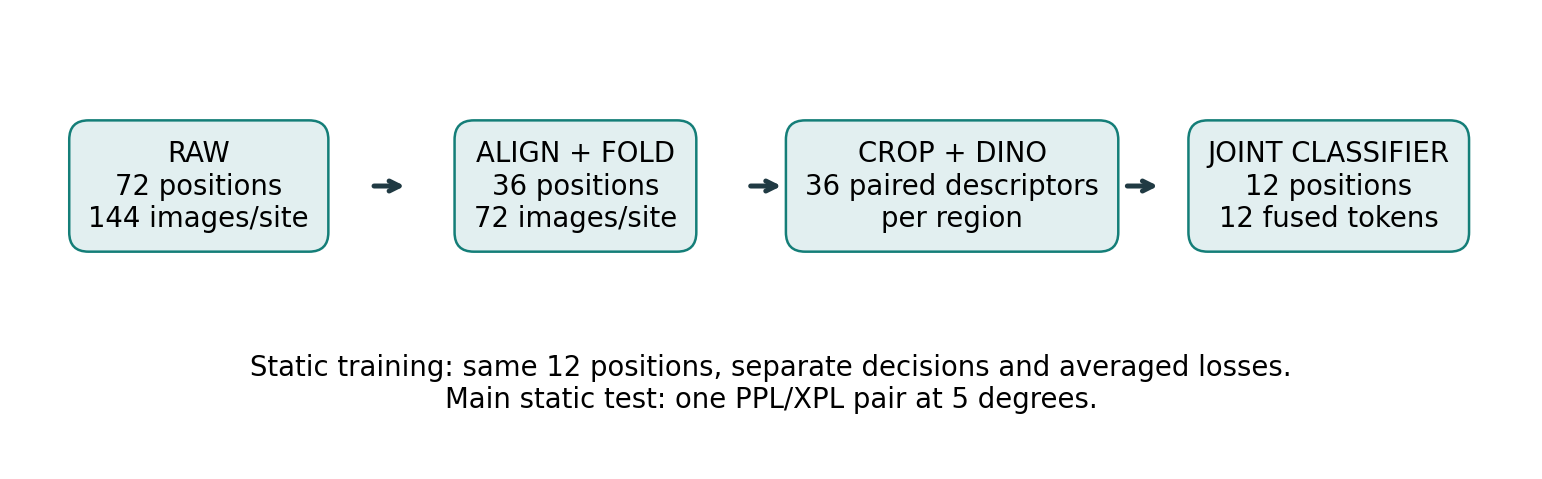
\includegraphics[width=\linewidth]{images/views_flow.png}
\vspace{0.6cm}
\textbf{Research question}\par
Does a classifier improve when it can inspect a region at multiple known microscope-stage angles instead of a single PPL/XPL pair?
\par\medskip
\textbf{What was done}\par
A processing and weak-labelling pipeline was built, followed by frozen DINOv2 image descriptors and three neural classification arms. Two training settings produced 120 full model fits across specimen-separated folds.
\par\medskip
\textbf{What was found}\par
The initial angle-aware and static models both achieved approximately 0.531 specimen-weighted macro-F1 against automatic singleton labels. The primary difference was indistinguishable from zero. Stronger regularisation did not establish a rotation advantage.
\vfill
\small These are results for classification given shared, automatically proposed regions and weak targets. They are not independently verified mineral-identification accuracy. Raw observations, reconstructed illustrations, historical GPU results, and proposed improvements are distinguished throughout.
\end{titlepage}
\pagenumbering{roman}
\tableofcontents
\clearpage
\pagenumbering{arabic}
\section{Research question and the meaning of the experiment}
\subsection{The geological motivation}
A thin section is a slice of rock made sufficiently thin for transmitted-light microscopy. A single section contains many mineral grains. Under plane-polarised light (PPL), useful observations include colour, absorption, texture and boundaries. Under cross-polarised light (XPL), brightness and interference colours can change as the stage rotates. Extinction is the dark orientation of an anisotropic grain between crossed polarisers. Pleochroism is a change in apparent colour or absorption with orientation in PPL.

The motivation is therefore straightforward: a geologist uses changing appearances, so a model might benefit from them too. However, more photographs do not automatically provide more independent information. A model also needs reliable alignment, appropriate regions, useful features, enough independent specimens and trustworthy evaluation targets.

\subsection{Questions tested}
\begin{enumerate}
\item \textbf{Primary:} under the same regions, descriptors, splits and target policy, does a 12-position angle-aware model outperform a single-position model?
\item \textbf{Secondary:} does knowing the angles help compared with a model seeing the same 12 positions without angle information?
\item \textbf{Diagnostic:} how much do target availability, class support, training instability and preprocessing restrict interpretation?
\end{enumerate}
The operational task is five-family classification. It is not full mineral-species identification, automatic discovery of every grain, or an independently validated replacement for a petrographer.

\subsection{Three kinds of evidence}
This report uses saved GPU predictions and evaluation files for quantitative outcomes; the current source snapshot for implementation explanations; and local images and masks for visual demonstrations. The historical GPU checkout and complete resolved regularised-run configuration were not archived together. Consequently, the current source is an explanatory snapshot, not a certified byte-for-byte copy of the historical training environment. Local regenerated label tables can differ from archived training evidence; historical counts below are taken from the run evidence.

There is no fresh training in preparing this report. The 72-position, unaveraged experiment is a proposed improvement, not a completed experiment. This separation prevents an implementation idea from being presented as a result.

\subsection{Vocabulary and units of independence}
\begin{tabularx}{\linewidth}{@{}lX@{}}
\toprule Term & Meaning in this project\\\midrule
Specimen & A rock sample identifier; the unit kept separate across train/test splits.\\
Site & A particular field of view within a specimen, such as \code{granite_r1}.\\
Stage position & One angle of microscope-stage rotation.\\
Image & One mode, PPL or XPL, at one position. Two images form a pair.\\
Region & A connected area proposed by segmentation; it need not equal one physical grain.\\
Weak target & A provisional family or allowed family set inferred from rules and metadata.\\
Embedding & A numerical image description produced by a frozen pretrained neural encoder.\\
Fold / seed & A specimen split / an initialisation and sampling randomisation.\\\bottomrule
\end{tabularx}
\takeaway{Thousands of images of a few rocks do not equal thousands of independent rock samples. The held-out specimen, rather than the image or grain, is central to evaluation.}

\section{Dataset provenance and organisation}
\subsection{Collection from the public Virtual Microscope}
The starting material comes from the public Virtual Microscope collection associated with The Open University \cite{ukvm}. It consists of existing microscope photographs and descriptive specimen metadata. The project did not capture these images with a local microscope.

The retained collection files indicate an automated download workflow: discover specimen records, resolve their viewer resources, enumerate rotation sites and PPL/XPL frame URLs, save images in a consistent hierarchy, and record failures and metadata. Viewer resource information and specimen indexes support this reconstruction. The original downloader, referenced in older documentation as \code{tools/ukvm_download.py}, is absent from the reviewed source tree. Its exact retry, throttling and URL-parsing implementation therefore cannot be asserted from this snapshot. The saved files establish what was downloaded more strongly than they establish every detail of the scraping procedure.

The relevant hierarchy is:
\begin{quote}\small\ttfamily
data/raw/ukvm\_dataset/\newline
\hspace*{1em}specimens.csv; rotation\_fields.csv; failures.csv\newline
\hspace*{1em}specimen\_index.json\newline
\hspace*{1em}specimens/<specimen>/\newline
\hspace*{2em}meta.json; viewer resources\newline
\hspace*{2em}rot/<site>/ppl/000.jpg ... 071.jpg\newline
\hspace*{2em}rot/<site>/xpl/000.jpg ... 071.jpg
\end{quote}
Original metadata and attribution must remain attached to redistributed material. Public access does not imply unrestricted reuse; collection-specific and third-party rights still apply. The companion repository excludes raw imagery and full data arrays. Figure provenance and image-rights notes are provided separately.

\subsection{How many observations are available?}
At a complete site the nominal raw angles are $0^\circ,5^\circ,\ldots,355^\circ$. Thus there are 72 positions and $72\times2=144$ photographs. Each image in this collection is approximately $490\times490$ pixels. PPL and XPL are different lighting observations, not duplicate copies.

\begin{table}[htbp]\centering
\caption{Data reduction and available supervision. Counts describe different units and should not be divided indiscriminately.}
\begin{tabularx}{\linewidth}{@{}rX@{}}\toprule Count & Stage / interpretation\\\midrule
115 & Specimens in the local Phase 0 inventory.\\
490 & Raw rotation folders before duplicate removal.\\
244 & Unique sites after removing 246 repeated folders.\\
242 & Sites meeting basic completeness and image checks.\\
233 & Sites passing alignment quality control.\\
22,389 & Automatically proposed regions in the segmentation collection.\\
5,065 & Regions represented in the archived full embedding run.\\
4,956 & Regions with pooled out-of-fold predictions; 112 specimens.\\
581 & Singleton-labelled test regions, from 77 specimens.\\
323 & Partial-set test regions, from 29 specimens.\\
4,052 & Predicted test regions whose teacher abstains.\\\bottomrule
\end{tabularx}
\end{table}
The difference between 5,065 and 4,956 is 109 mixed/excluded regions (66 mixed and 43 excluded in the archived accounting). Of the 4,956 predicted regions, only 904 have singleton or partial-set supervision. A large prediction count therefore does not imply a large labelled benchmark.

\subsection{Phase 0: clean the collection before measuring it}
Phase 0 builds an explicit inventory. It checks required files, decodability, consistent dimensions and completeness. Duplicate-site detection uses selected reference files, including PPL frame 000, XPL frame 000 and PPL frame 037, within a specimen. This removes exact repeated sites without intentionally merging distinct specimens. A hash of representative frames is an engineering duplicate check, not proof that every near-duplicate has been found.

The resulting \code{sites.csv} contains canonical site identifiers and usability information; \code{specimens_clean.csv} normalises specimen records. Missing image/whole-slide resources and incomplete sites are documented in the report. Two unusable sites in the inventory are \code{glahm134751_r2} and \code{lun35_r5}. An adjacent-frame PPL exposure-change check flags a relative jump above approximately 15\%; this is a warning rather than an automatic mineral classification. One site, \code{watson389_r2}, receives this flag.

The metadata include rock type and reported constituent minerals. These describe a \emph{specimen}. They do not identify the mineral occupying an individual pixel or region. Monomineralic flags were retained for description, but the V1 policy does not use a rock title alone to assign every region that mineral.

\subsection{Spatial calibration}
Scale information was estimated from whole-slide scale metadata and the relationship between whole-slide and rotation views. In simplified form,
\begin{equation}
u_{\rm rot}=\frac{1000}{\text{whole-slide pixels per mm}}
\times d_{\rm saved}\times s_{\rm rot\to WSI},
\end{equation}
where $u_{\rm rot}$ is micrometres per rotation-image pixel, $d_{\rm saved}$ accounts for saved-image downsampling, and $s_{\rm rot\to WSI}$ is the measured registration scale. Ten calibration specimens yielded a median near $4.181\,\mu$m/pixel and a coefficient of variation near 0.9\%. A 490-pixel image width is therefore about 2.05 mm under this approximation. The 464-pixel valid-circle diameter is about 1.94 mm.

This approximate spatial scale helps interpret grain sizes. It does not calibrate brightness, exposure, thin-section thickness or birefringence. Those are separate measurements.

\fig{raw.png}{1}{Running example: raw photographs from \code{granite_r1}. The spatial structures rotate while optical appearance also changes. The source photographs originate from the Virtual Microscope collection; this layout is a project illustration.}{fig:raw}
\FloatBarrier

\section{Phase 1: put the same region at the same pixels}
\subsection{Why registration is necessary}
Without registration, pixel $(x,y)$ at one angle can describe a different part of the rock at the next angle. A brightness curve would then mix motion with mineral optics. Phase 1 estimates a geometric transformation for every frame relative to frame 0. The transformation estimated from PPL is also applied to the corresponding XPL image. This assumes the PPL and XPL pair share acquisition geometry.

\subsection{ORB: finding and describing repeatable landmarks}
ORB stands for \emph{Oriented FAST and Rotated BRIEF} \cite{orb}. It is a feature detector and descriptor, not a mineral classifier. FAST identifies corner-like intensity patterns. Conceptually, a point is distinctive when a contiguous arc on a small surrounding circle is consistently brighter or darker than its centre by a threshold. Such local corners are often easier to match than smooth, uniform interiors.

ORB estimates a local orientation using intensity moments. For coordinates relative to the patch centre,
\begin{equation}
m_{pq}=\sum_{x,y}x^p y^q I(x,y),\qquad
\alpha=\operatorname{atan2}(m_{01},m_{10}).
\end{equation}
BRIEF then compares intensities at selected point pairs. Each comparison produces a bit,
\begin{equation}
b_j=\mathbf{1}\{I(\mathbf u_j)<I(\mathbf v_j)\}.
\end{equation}
Rotating the sampling pattern by $\alpha$ makes the descriptor less sensitive to image rotation. Two descriptors are compared using Hamming distance: the number of disagreeing bits, $d_H(b,b')=\sum_j\mathbf{1}\{b_j\ne b'_j\}$. The pipeline requests up to 3,000 ORB keypoints, uses cross-checked brute-force Hamming matches, retains at most 600 good matches and requires at least 10 correspondences for the registration attempt.

This works when repeatable geometry remains visible. It becomes unreliable in feature-poor areas, at changing contrast, or when many apparently similar textures produce incorrect correspondences. A match is a proposal, not automatically a correct link.

\subsection{RANSAC: reject geometrically inconsistent matches}
The fitted transform is a 2-D similarity transform,
\begin{equation}\label{eq:similarity}
\begin{bmatrix}x'\\y'\end{bmatrix}
=\begin{bmatrix}a&-b\\b&a\end{bmatrix}
\begin{bmatrix}x\\y\end{bmatrix}
+\begin{bmatrix}t_x\\t_y\end{bmatrix},\qquad
s=\sqrt{a^2+b^2},\quad\varphi=\operatorname{atan2}(b,a).
\end{equation}
It allows rotation, uniform scale and translation, rather than an unrestricted deformation of a grain. RANSAC (random sample consensus) repeatedly fits candidate transformations from small subsets of matches \cite{ransac}. For match $j$, the reprojection residual is
\begin{equation}
r_j=\|T\mathbf x_j-\mathbf x'_j\|_2.
\end{equation}
Matches with $r_j\leq2$ pixels count as inliers for the configured fit. The model supported by a consistent set is retained and refined. In ideal independent sampling, if $w$ is the inlier fraction and $m$ the minimal subset size, the number of draws needed for success probability $p$ satisfies
\begin{equation}
N\geq\frac{\log(1-p)}{\log(1-w^m)}.
\end{equation}
This explains why many bad matches make robust fitting harder. It is an explanation of RANSAC, not a claim that the project manually fixes $N$ using this formula.

The estimated angle is checked against the nominal stage rotation: allowed error is about $1.5^\circ$ for a candidate transform, and scale must remain within about 1\% of unity. Rotation sign is inferred from early frames, with a default if no early estimate succeeds. Sign conventions depend on whether the transform maps the moving frame to the reference; physical stage rotation and image correction need not have the same sign.

\subsection{Fallbacks, refinement and valid support}
Registration first tries a direct reference match. If that fails, it can compose a match through a neighbouring frame. If this also fails, it uses nominal rotation around the image centre. The fallback provides a usable guess, but its presence must remain visible in quality control.

An enhanced correlation coefficient (ECC) refinement follows the coarse alignment \cite{ecc}. Conceptually, it optimises normalised correlation between centred image signals,
\begin{equation}
\rho(\mathbf p)=\frac{\widetilde I_{\rm ref}^{\mathsf T}\widetilde I_{\rm mov}(W(\mathbf p))}
{\|\widetilde I_{\rm ref}\|\,\|\widetilde I_{\rm mov}(W(\mathbf p))\|}.
\end{equation}
The implementation uses gradient images and an Euclidean residual warp. Gradients emphasise changes at structures rather than absolute brightness. The residual transform is composed with the coarse warp using the appropriate inverse-warp convention. This is an optimisation step, not an independent proof of correct registration.

Interpolation samples a rotated image on the reference pixel grid. It can soften edges. A valid mask is obtained by warping support masks, intersecting support across frames and restricting it to the configured circle. Black corners after rotation are invalid support, not opaque minerals.

\subsection{Opposite-angle averaging: what was actually done}
For each illumination mode separately, the aligned stack is folded:
\begin{equation}\label{eq:fold}
\bar I_k=\operatorname{round}\left[\frac{I^{\rm aligned}_k+I^{\rm aligned}_{k+36}}2\right],
\quad k=0,\ldots,35.
\end{equation}
The calculation is performed in floating point before conversion to the saved image type. PPL is averaged with PPL; XPL with XPL. It does \emph{not} average PPL and XPL together. The resulting 36 retained positions each have two pictures: 36 PPL images and 36 XPL images, hence 72 images total.

Ideal orientation-dependent optical responses can repeat after a half-turn. For example, a simple crossed-polariser intensity law has a $\sin^2(2\theta)$ factor, and absorption terms can have a $\cos(2\theta)$ dependence. These motivate testing half-turn folding. They do not establish that acquired image pairs are identical: drift, JPEG compression, illumination changes, deformation and residual misalignment can violate the assumption. Averaging can reduce independent noise, but can also blur structure or erase useful acquisition differences. A no-averaging ablation is required to determine its effect here; it has not been completed.

Frame 0 has a special interpolation history: its folded image averages the original reference with a resampled opposite frame, whereas most other retained positions combine two resampled frames. The main static test uses $5^\circ$ to avoid this particular reference-frame advantage. It does not remove every possible preprocessing asymmetry.

\subsection{Alignment quality control and the edge image}
The current code's site-level pass condition is stricter than its individual-transform acceptance check:
\begin{align}
\operatorname{median}(|\text{angle error}|)&<0.5^\circ, & n_{\rm fallback}&<3,\\
\text{residual shift}&<0.3\text{ pixels}, & \text{opposite-frame difference}&<10.
\end{align}
The difference is the mean absolute grayscale difference between aligned $0^\circ$ and $180^\circ$ PPL frames after a light Gaussian blur, within valid support. Residual translation uses gradient phase correlation. These checks are proxies: they do not validate every point in every frame. In the saved collection, 233 of 242 usable sites pass.

\fig{align.png}{1}{Phase 1 QC for \code{granite_r1}. The first panels show registered PPL observations. In the edge overlay, red represents edges at $0^\circ$ and green those at $90^\circ$. Coincident red and green appear yellow. Separated double edges suggest residual mismatch; a changed optical contrast can also make an edge appear in only one colour.}{fig:align}
The overlay is useful because the eye readily notices doubled contours. It is not an error map with a calibrated pixel value, and red does not mean a particular mineral. Boundary disagreement should be checked against the images and numerical residuals together.
\FloatBarrier

\section{Phase 2: convert angle-dependent appearance into maps}
\subsection{Optical motivation versus measured image values}
For an ideal transparent anisotropic section between crossed polarisers, a simplified monochromatic relation is
\begin{equation}\label{eq:optics}
I(\theta,\lambda)\propto I_0(\lambda)\sin^2[2(\theta-\theta_e)]
\sin^2\left(\frac{\pi\Delta n\,t}{\lambda}\right),
\end{equation}
where $\Delta n$ is effective birefringence, $t$ thickness, $\lambda$ wavelength and $\theta_e$ an extinction orientation. This ideal relation motivates the fourth angular harmonic, because $\sin^2(2\theta)=(1-\cos4\theta)/2$. Real RGB photographs integrate wavelengths and include camera response, exposure and compression.

The implemented luminance proxy is $Y=0.299R+0.587G+0.114B$ on encoded RGB values. It is not calibrated linear radiance. A white reference $W$ is estimated from the bright PPL distribution; bright neutral pixels support channel balancing. These full-sequence quantities are used in optical maps and region proposals. They must not be described as calibrated mineral constants, nor as the fixed normalisation applied to the neural crops.

\subsection{XPL extinction position, anisotropy and fit quality}
At a valid pixel, let $Y_k$ be XPL luminance at retained angle $\theta_k$, in radians. For $N=36$ evenly spaced samples,
\begin{align}
\mu &= N^{-1}\sum_kY_k,\\
c_4 &= \frac{2}{N}\sum_kY_k\cos(4\theta_k), &
s_4 &= \frac{2}{N}\sum_kY_k\sin(4\theta_k),\\
\widehat Y(\theta)&=\mu+c_4\cos4\theta+s_4\sin4\theta.
\end{align}
Write $A_4=\sqrt{c_4^2+s_4^2}$ and $\phi=\operatorname{atan2}(s_4,c_4)$. The fitted dark position is
\begin{equation}
\theta_e=\frac{\phi+\pi}{4}\pmod{\pi/2}.
\end{equation}
Extinction is represented modulo $90^\circ$, because this model repeats every quarter-turn. The normalised modulation and fit score are
\begin{equation}
a=\operatorname{clip}\left(\frac{A_4}{\mu+1},0,1\right),\qquad
R_4^2=\operatorname{clip}\left(\frac{A_4^2/2}{\operatorname{Var}(Y)},0,1\right).
\end{equation}
The variance denominator uses the same equally sampled observations; constant curves receive a zero score rather than division by zero. This expression corresponds to the variance explained by the harmonic on that grid. The additive 1 stabilises dark pixels and is an image-unit choice.

Large $a$ means strong relative oscillation. Large $R_4^2$ means the fourth harmonic explains much of the observed variation. Neither by itself identifies a mineral. The anisotropic-pixel mask requires approximately $a\geq0.15$, sufficient XPL brightness ($\max Y\geq0.08W$), and valid support. Low brightness can make an angle estimate unstable even if a ratio appears large.

Two different bright-XPL representations are retained. A maximum projection takes per-channel maxima across angles and may combine colours that never coexisted in one photograph. A fitted bright-position representation samples near $\theta_e+45^\circ$ and $\theta_e+135^\circ$. The names should not be interchanged.

\subsection{PPL colour change and other descriptors}
PPL luminance is fitted with the second harmonic,
\begin{equation}
\widehat Y_{\rm PPL}(\theta)=\mu+c_2\cos2\theta+s_2\sin2\theta.
\end{equation}
The dark absorption direction is $(\operatorname{atan2}(s_2,c_2)+\pi)/2$ modulo $\pi$. Channel-wise fits estimate colours at opposite absorption states separated by $90^\circ$. Their CIELAB distance is
\begin{equation}
\Delta E_{76}=\sqrt{(L_1^*-L_2^*)^2+(a_1^*-a_2^*)^2+(b_1^*-b_2^*)^2}.
\end{equation}
This is a repeatable colour-change descriptor, not a spectroscopic measurement. Lighting and registration can contribute to it. Other maps include a dark-PPL opaque candidate mask ($\max Y_{\rm PPL}<0.15W$), local texture and a modulation of gradient magnitude sometimes described as relief or twinkling. The latter can respond to several causes and is not a specific carbonate test.

The code also contains a Michel--L\'evy-inspired colour-to-retardation approximation using $\Gamma=\Delta n\,t$. With unknown relative PPL/XPL exposure, section thickness and colour response, such a lookup is not a reliable measurement of $\Delta n$. Birefringence is disabled as a deciding term in V1 labelling. Its presence in a saved table does not imply it was trusted as a V1 target criterion.

\fig{maps.png}{1}{Phase 2 maps for \code{granite_r1}. Top: reference PPL, reference XPL and an XPL maximum projection. Bottom: fitted extinction position (cyclic colour), relative XPL modulation, and PPL colour change. These original QC panels lack numerical colour bars; read them qualitatively, not as calibrated scales. A coloured boundary may indicate a changed optical response, not necessarily a separate grain or a different mineral.}{fig:maps}
\fig{optical_curves.png}{0.94}{Reconstructed region-mean curves for two example masks. Dots/solid lines are mean luminance from the local folded stack; dashed lines fit the corresponding second or fourth harmonic. These averages illustrate angular behaviour. They are not the per-pixel map fits, not historical neural inputs exported from the GPU cache, and not new ground-truth measurements.}{fig:curves}
\takeaway{Phase 2 asks ``how does this location change?'' It provides measurable descriptors for later steps, not a coloured mineral-identification image.}
\FloatBarrier

\section{Phase 3: propose regions rather than assume known grains}
\subsection{Feature space and initial superpixels}
Segmentation groups pixels into candidate regions. It uses appearance and optical behaviour together. The eight-dimensional pixel feature vector is approximately
\begin{equation}
\mathbf f(x)=\left[\operatorname{Lab}(I_{\rm XPL,max}),\;
0.7\operatorname{Lab}(I_{\rm PPL,mean}),\;
40a\cos4\theta_e,\;40a\sin4\theta_e\right].
\end{equation}
There are three XPL colour values, three PPL colour values, and two angular values. A median filter suppresses small isolated fluctuations. Encoding angles with sine and cosine avoids an artificial discontinuity between extinction positions near $0^\circ$ and $90^\circ$; multiplying by $a$ reduces the influence of an uncertain angle at a weakly varying pixel.

SLIC (simple linear iterative clustering) makes compact initial superpixels \cite{slic}. Conceptually, its distance balances feature similarity and spatial proximity,
\begin{equation}
D^2=d_f^2+\left(\frac{m}{S}\right)^2d_{xy}^2,
\end{equation}
where $S$ is an approximate superpixel spacing and $m$ controls compactness. The implementation targets approximately 60 pixels per initial superpixel with compactness 5. These are algorithmic seeds, not final mineral grains.

\subsection{Neighbour merging and postprocessing}
A region adjacency graph connects touching superpixels. Neighbours with similar mean feature vectors are merged hierarchically; the configured distance threshold is 18. If regions $A$ and $B$ merge, their mean feature updates as
\begin{equation}
\overline{\mathbf f}_{A\cup B}=\frac{|A|\overline{\mathbf f}_{A}+|B|\overline{\mathbf f}_{B}}{|A|+|B|}.
\end{equation}
This accumulates local evidence, but can merge two similar minerals or split one heterogeneous grain. A further twin-domain merging heuristic considers PPL colour similarity, an approximate birefringence-class difference, boundary evidence and shared boundary length. The configured checks include PPL $\Delta E<6$, class difference at most 1, boundary ratio below 0.5 and at least 15 shared boundary pixels. Very small components around 150 pixels are merged; regions below approximately 400 pixels can be marked small.

An important distinction is that unreliable birefringence was disabled in V1 \emph{labelling}, while the pre-existing frozen segmentation can still reflect its earlier merging heuristic. Removing a term from the teacher does not retrospectively remove every influence of that term from preprocessing.

\subsection{Why boundaries can look wrong}
Several effects explain the suspicious contours noticed during visual review:
\begin{itemize}
\item Twins, alteration, cracks and extinction domains can divide one physical crystal into several appearance regions.
\item Similar adjacent grains can merge when colour and optical summaries are insufficiently different.
\item Residual registration mixes pixels near an edge, changing both maps and later boundaries.
\item The common valid circle is an acquisition mask. Its edge is not the edge of a mineral, and need not follow the full bright circular field in an individual image.
\item SLIC and graph thresholds impose resolution choices; small fragments can be algorithmic rather than geological.
\end{itemize}
V1 freezes these regions to keep identities and splits stable while comparing classifiers. This provides a controlled comparison on shared regions, not a claim of perfect segmentation. No expert-mask intersection-over-union benchmark is available in the reviewed results.

\fig{segment.png}{1}{Yellow outlines from the same segmentation mask over PPL and XPL context. The long central structures contain internal optical and textural changes; an outline following those changes is not automatically a true grain boundary. The outer yellow contour also reflects valid support.}{fig:segment}
\FloatBarrier

\section{Phase 4: write a property record for each region}
\subsection{Geometry, erosion and eligibility}
For each region the feature table stores its area, centroid, bounding box, aspect ratio and edge/partial status. The interior is eroded by two pixels before many optical summaries are measured. Erosion removes a narrow boundary band where alignment errors and mixed pixels are most likely. It trades some data for more stable measurements.

The V1 geometric gate requires at least 1,000 region pixels and at least 400 interior pixels. A partial region is not automatically excluded if usable interior evidence remains. Habit and long-axis-related descriptors can be unresolved for partial or nearly equant regions. Large size alone does not guarantee that a region contains only one mineral.

\subsection{Robust and circular summaries}
Region medians reduce sensitivity to isolated pixels. The optical-class decision uses the proportion of opaque and anisotropic pixels: a region is opaque when its opaque fraction exceeds 0.8; otherwise an anisotropic fraction below 0.2 produces an isotropic-like category, and the remaining case is anisotropic. These are measured categories under the image model, not definitive mineral identities. An anisotropic region also needs a median fit score around $R_4^2\geq0.4$ to pass the relevant V1 quality check; opaque/isotropic cases cannot be judged by the same oscillation requirement.

Angles require circular statistics. Ordinary averaging of $1^\circ$ and $89^\circ$ would incorrectly suggest $45^\circ$ even though they are nearby modulo $90^\circ$. With modulation weights $a_j$,
\begin{equation}
z=\frac{\sum_j a_j e^{i4\theta_{e,j}}}{\sum_j a_j},\qquad
\overline\theta_e=\frac{\arg z}{4}\pmod{\pi/2},\qquad R=|z|.
\end{equation}
A concentration-derived spread is $\sigma_e=\sqrt{-2\log R}/4$, in radians, with suitable protection at numerical extremes. Low $R$ indicates inconsistent orientations or domains. PPL absorption directions use the second harmonic because they repeat modulo $180^\circ$.

The median PPL colour-change descriptor is categorised with thresholds near 4, 10 and 20: none, weak, moderate and strong. Such thresholds are practical heuristics, not universal boundaries between minerals.

\subsection{Twins, undulose response and measurement status}
Twin detection seeks coherent extinction domains among sufficiently reliable pixels. It checks domain size, separation and internal spread, together with PPL boundary behaviour. Example settings include pixel fit quality at least 0.5, domain fraction at least 0.1, angular separation around $8^\circ$ and within-domain spread around $7^\circ$. These checks try to distinguish optical domains from arbitrary texture. They have not been independently validated against a labelled twin dataset.

An undulose descriptor measures spatial variation in the circular extinction field through derivatives of $\cos4\theta_e$ and $\sin4\theta_e$. An ideal differential identity is
\begin{equation}
\|\nabla\theta_e\|=\frac14\sqrt{\|\nabla\cos4\theta_e\|^2+\|\nabla\sin4\theta_e\|^2}.
\end{equation}
The implementation uses Sobel derivatives and an empirical scale factor. Because the discrete Sobel response is not fully normalised into a physical spatial derivative, the saved number should be treated as an empirical descriptor, even where an older name suggests degrees per ten pixels. It is not a direct crystallographic strain measurement.

Each measurement can carry a status: \emph{observed}, \emph{not detected with a bound}, \emph{unresolved}, \emph{invalid}, or \emph{not applicable}. This prevents a missing or unmeasurable cue from being silently interpreted as a valid zero. For example, ``twins not measurable'' is different from ``a reliable search found no twins.''

\section{Phases 5 and 6: convert evidence into weak targets}
\subsection{Knowledge representation}
The knowledge directory supplies four complementary resources. \code{minerals.csv} describes expected properties; \code{aliases.csv} normalises alternative names; \code{hierarchy.yaml} connects species and families; \code{likelihoods.yaml} assigns heuristic evidence weights and compatibility values. Phase 5 checks that these resources load consistently. It does not fit a neural network.

The V1 output vocabulary contains five families:
\begin{table}[htbp]\centering
\begin{tabularx}{\linewidth}{@{}lX@{}}\toprule Output & Intended grouping and caveat\\\midrule
quartz & Quartz family; weak optical support and limited specimen support.\\
feldspar & Plagioclase, orthoclase, microcline and sanidine grouped together.\\
mica & Biotite and muscovite in the ontology; observed positive support is effectively biotite-heavy.\\
pyroxene & Augite and orthopyroxene grouped together.\\
opaque\_material & A dark-material category, not a single mineral species.\\\bottomrule
\end{tabularx}
\caption{The five predicted categories. Other plausible minerals remain relevant to rejection, even though they are not output classes.}
\end{table}
Amphibole, carbonate, tourmaline, olivine and garnet are among alternatives considered by the wider candidate registry. A classifier with five output categories cannot correctly name every possible mineral in a rock.

\subsection{Heuristic evidence scoring}
For candidate mineral $m$, features $f_j$ contribute weighted compatibility scores:
\begin{equation}
\ell_m=\sum_{j\in\mathcal O}w_j\log L_j(f_j\mid m),\qquad
p_m=\frac{\exp\ell_m}{\sum_{m'}\exp\ell_{m'}}.
\end{equation}
Here $\mathcal O$ is the set of usable deciding terms, and $L_j$ is a table-based or rule-based compatibility value. Family mass sums the probabilities of member minerals. An unlisted alternative receives a background compatibility (configured around 0.25 per active weighted term), and out-of-scope mass can trigger abstention.

This resembles a likelihood model but is not a calibrated probability of geological truth. The features are correlated, likelihood values are hand specified, and priors and metadata restrictions affect the normalisation. A score of 0.8 should not be presented as experimentally demonstrated 80\% mineral correctness.

\subsection{What a target is allowed to say}
The target policy uses both quality checks and informative positive evidence. An output family must have a positive cue that helps distinguish it from a relevant alternative; mere absence of contradiction is insufficient. The configured decisions are approximately:
\begin{enumerate}
\item Exclude inadequate measurements; flag fine aggregates as mixed rather than singleton grains.
\item Abstain if out-of-scope mass is at least 0.2 or hard optical contradictions remain.
\item Assign a singleton if the winning in-scope family mass reaches 0.8 and the positive-evidence requirements pass.
\item Otherwise allow a set of at most two families if its cumulative mass reaches 0.9 and the checks pass.
\item Abstain when evidence remains diffuse or unsupported.
\end{enumerate}
These states have different meanings:
\begin{quote}
\textbf{Singleton:} ``the teacher accepts mica.''\quad
\textbf{Partial set:} ``the teacher accepts quartz or feldspar.''\quad
\textbf{Abstain:} ``the teacher cannot provide a usable target.''\quad
\textbf{Mixed/excluded:} unsuitable for the supervised region task under this policy.
\end{quote}
An abstaining region may still receive a neural prediction for inspection. That prediction does not acquire a ground-truth label merely because the network produces a confident softmax output.

\subsection{Metadata dependence and circular evaluation}
The teacher is evaluated with optical evidence alone and with specimen mineral lists restricting alternatives. A target receives \code{metadata_dependent} when its state or allowed set changes between these conditions. Metadata can remove alternatives and thereby sharpen a target. It is not supplied as an input token to the neural classifier, but it affects what the classifier learns and what it is scored against.

In the archived out-of-fold singleton set, all 537 non-opaque singleton targets are metadata-dependent. The remaining 44 targets are opaque material. This means the experiment primarily measures recovery of a teacher that combines optical heuristics and specimen context. It does not establish independent mineral truth. A check counting predictions outside a specimen's list is useful for consistency, but provides weak independent validation when that same list helped create the targets.

The V1 deciding-term exclusions include birefringence, extinction type, relief, cleavage and absorption axis. Disabling these unreliable or insufficiently validated terms reduces unsupported certainty, but also removes information the earlier teacher used. A separately named twinkling term is present in the rules and should not be confused with the disabled relief term; it remains an empirical cue requiring validation. Rock-title or monomineralic assignment alone is not accepted as evidence for every region.

\subsection{Fold-local thresholds and feasibility checks}
Data-derived cutoffs, including undulose and twinkling quantiles, are fitted using training specimens for each fold and then frozen. Nominal quantiles are the 80th and 90th percentiles respectively. This prevents test specimens from determining those thresholds. Hand-written choices made during project development and full-sequence preprocessing still impose other limitations; fold-local fitting is not a blanket guarantee against every source of bias.

Before neural training, a feasibility gate checks target files, required status columns, prohibited deciding terms, aggregate handling and class support. Each class must have at least five singleton training specimens in every fold. Passing this gate means the planned experiment is operationally feasible. It does not certify label accuracy or adequate statistical power.

\section{Phase 7: assemble a specimen-separated learning dataset}
\subsection{Splits and class support}
The split unit is the specimen. All sites and regions from one specimen stay together. Five grouped folds are stratified approximately by rock family, with very rare families pooled into an ``other'' stratum. Within each training portion, approximately 15\% of specimens are reserved for validation with a fixed random seed. Frozen split files and their hashes protect against accidental reassignment.

The held-out singleton support is uneven:
\begin{table}[htbp]\centering
\begin{tabular}{@{}lrr@{}}\toprule Family & Regions & Specimens containing targets\\\midrule
Quartz & 99 & 12\\
Feldspar & 160 & 37\\
Mica & 142 & 16\\
Pyroxene & 136 & 23\\
Opaque material & 44 & 20\\\bottomrule
\end{tabular}
\caption{Archived pooled out-of-fold singleton support. Specimen columns overlap across classes and must not be summed as unique specimens.}
\end{table}
Quartz's 12 specimens make its held-out estimate especially uncertain. A fold can pass the training-support gate while its validation set lacks a class; fold 4's validation set has no quartz singleton in the reviewed evidence.

\subsection{Crops and fixed geometry}
Each region has a square crop centred on its bounding box. The approximate side length is
\begin{equation}
L=\max\{48,\operatorname{round}[1.3\max(w,h)]\}.
\end{equation}
The same crop geometry is used for all retained angles and both modes. Images are resized to $224\times224$ pixels; masks use nearest-neighbour resizing. Pixels outside the selected region are dimmed to 35\% intensity, rather than erased completely, to preserve limited context. This also leaves a possible context shortcut, so good performance need not mean the model relies exclusively on the grain interior.

All arms share masks and regions built using rotational information. Thus the comparison asks about \emph{classification given shared regions}. It is not a comparison between a completely single-image pipeline and a completely rotational pipeline. This qualification is central to any interpretation of a gain or a lack of gain.
\FloatBarrier

\section{Phase 8: frozen DINOv2 image descriptions}
\subsection{What DINOv2 contributes}
DINOv2 is a vision transformer pretrained through self-supervised learning on a large image collection \cite{dinov2}. During its original pretraining, related views of images provide learning signals without requiring mineral labels. RotaPetro uses the pretrained encoder as a fixed feature extractor. It does not train DINOv2 from scratch on thin sections, and the reviewed V1 run does not fine-tune its weights.

The selected encoder is ViT-S/14. A $224\times224$ crop is divided into $14\times14$ patches, giving a $16\times16$ grid of 256 patch tokens. Each patch token and the global classification (CLS) token have dimension 384. A patch token describes local visual content; the CLS token summarises the image in the pretrained representation.

Input channels are scaled from integer RGB to $[0,1]$, then normalised using fixed ImageNet means $(0.485,0.456,0.406)$ and standard deviations $(0.229,0.224,0.225)$. This differs from normalising each site using its full angle sequence. The latter would give the static model information from unseen angles; it is not the intended crop normalisation here.

\subsection{Mask-weighted pooling}
Let $\mathbf t_j\in\mathbb R^{384}$ be the DINO patch token and $q_j\in[0,1]$ the fraction of patch $j$ covered by the resized region mask. The local region description is
\begin{equation}
\mathbf e_{\rm region}=\frac{\sum_{j=1}^{256}q_j\mathbf t_j}{\sum_{j=1}^{256}q_j+\epsilon},\qquad
\mathbf e=[\mathbf e_{\rm CLS};\mathbf e_{\rm region}]\in\mathbb R^{768}.
\end{equation}
The mask makes the pooled descriptor focus more strongly on the selected region. The CLS half still contains crop context. This pair of global and local summaries is stored for each PPL and XPL crop.

The archived cache represents 5,065 regions, one stored version, 36 retained positions, two modes and 768 features per image:
\begin{equation}
E\in\mathbb R^{5065\times1\times36\times2\times768}.
\end{equation}
It is stored in half precision. All 36 positions are encoded once to make comparisons efficient; this does not mean the classifier jointly sees all 36 on each decision. No additional geometric augmentation versions are present in that cache.

\subsection{Why DINO could help or hinder}
Generic visual features can recognise texture, colour, edges and shape with few project-specific targets. Freezing them makes training fast and reduces the number of parameters fitted from a small label set. On the other hand, subtle extinction or colour trajectories may not survive its pretrained invariances or region pooling. The current results contain no encoder ablation or fine-tuning comparison. They cannot identify DINO as the bottleneck. That hypothesis needs a controlled comparison against optical descriptors, other frozen representations and carefully supervised fine-tuning.

\section{Phase 9: compare three neural decision rules}
\subsection{What each arm receives}
\begin{table}[htbp]\centering
\begin{tabularx}{\linewidth}{@{}lXX@{}}\toprule Arm & Training decision & Main test decision\\\midrule
Static & Each of the same 12 chosen positions is processed independently; average the 12 losses. & One PPL/XPL pair at $5^\circ$.\\
Unordered multi-view & Jointly process 12 paired positions without angle encoding. & Positions $5^\circ,20^\circ,\ldots,170^\circ$, no angle encoding.\\
Angle-aware multi-view & Jointly process those 12 paired positions with explicit angular features. & The same 12 positions with angular features.\\\bottomrule
\end{tabularx}
\caption{Controlled view comparison. All arms use the same frozen encoder, targets, specimen splits and selected training views.}
\end{table}
During training, indices are $k_j=(o+3j)\bmod36$, for $j=0,\ldots,11$. The offset $o$ changes deterministically with seed, epoch and region so different retained angles can contribute across epochs. At validation and test, the multi-view indices are $1,4,7,\ldots,34$ and the static index is 1. Static validation therefore also uses the designated single position; it is not a 12-position ensemble.

Equal exposure to selected training pictures addresses a simple unfairness: the multi-view model should not win merely because it alone was trained on varied angles. The models still solve different decision tasks: one image pair at a time versus joint evidence from twelve. Parameter counts and validation-loss behaviour are similar but not identical.

\subsection{Mode fusion and tensor shapes}
For position $k$, let $\mathbf e_k^P,\mathbf e_k^X\in\mathbb R^{768}$ be PPL/XPL descriptors. Learned linear projections fuse the pair:
\begin{equation}
\mathbf z_k=\operatorname{LayerNorm}\big(W_P\mathbf e_k^P+W_X\mathbf e_k^X+\text{bias terms}\big)
\in\mathbb R^{256}.
\end{equation}
There is \emph{one fused token per position}. Twelve positions supply 24 image descriptions but 12 fused tokens. With the learned sequence CLS token, the transformer receives 13 tokens, not 24 or 144. The static model receives one fused token plus CLS.

\subsection{Angle encoding is already implemented}
The angle-aware model adds
\begin{equation}
\mathbf a(\theta)=\operatorname{MLP}\left[
\sin2\theta,\cos2\theta,\sin4\theta,\cos4\theta\right],
\qquad \mathbf z'_k=\mathbf z_k+\mathbf a(\theta_k),
\end{equation}
where the MLP maps $4\to64\to256$ dimensions with GELU nonlinearity. Harmonics encode periodic relationships without a discontinuity at the cycle boundary. They are physics-motivated coordinates, not a hard constraint enforcing the optical intensity law.

This is angular sequence modelling, not elapsed-time forecasting. The current project already tests explicit angle awareness. Adding the phrase ``temporal model'' without changing the data or architecture is not a new experiment. Also, the selected harmonics repeat after $180^\circ$: a future full-turn model should examine whether it needs $\sin\theta,\cos\theta$ or other encodings to distinguish opposite positions while retaining physical periodicity features.

\subsection{How attention combines observations}
For a sequence matrix $Z$, self-attention forms queries, keys and values,
\begin{equation}
Q=ZW_Q,\quad K=ZW_K,\quad V=ZW_V,\qquad
\operatorname{Attention}(Q,K,V)=\operatorname{softmax}\left(\frac{QK^{\mathsf T}}{\sqrt{d_h}}\right)V.
\end{equation}
The dot products measure learned compatibility between observations. The weighted sum allows the representation of one position to use evidence from another. Multiple heads use different learned projections \cite{attention}. The reviewed classifier uses two pre-layer-normalised transformer layers, four heads, 256-dimensional tokens and a 512-dimensional feed-forward sublayer with GELU. Each head has 64 features. Residual connections preserve the incoming representation while adding attention and feed-forward updates.

The final representation concatenates sequence CLS with the mean of the position tokens. The resulting 512 values pass through a $512\to256\to5$ classification head. Softmax produces five probabilities,
\begin{equation}
p_c=\frac{e^{u_c}}{\sum_{j=1}^{5}e^{u_j}}.
\end{equation}
These are model scores over five available outputs. Without confidence calibration and an unknown-class policy, a high maximum does not guarantee correctness or exclude an unmodelled mineral.

The unordered arm has no positional/angle embedding. Its attention operations are permutation equivariant and its pooled prediction is permutation invariant in evaluation. This does not require the data loader to explicitly shuffle the tokens. The angle-aware arm attaches angular content to each observation rather than relying on an arbitrary file order.

\subsection{Learning with singleton and partial-set targets}
For allowed class set $S_i$, the supervised loss is
\begin{equation}\label{eq:setloss}
\mathcal L_i=-\log\sum_{c\in S_i}p_{ic}.
\end{equation}
For a singleton this becomes ordinary cross-entropy, $-\log p_{iy_i}$. For $S_i=\{\text{quartz},\text{feldspar}\}$, the loss rewards total mass on either family without pretending to know which is correct. It does not impose a 50/50 target. Empty sets and unsuitable states do not provide this supervised signal.

For the static arm, the region's training loss averages independent decisions,
\begin{equation}
\mathcal L_i^{\rm static}=\frac1{12}\sum_{k\in\mathcal K_i}
-\log\sum_{c\in S_i}p(c\mid\mathbf e_{ik}^P,\mathbf e_{ik}^X).
\end{equation}
For multi-view arms, one set loss is calculated after the joint sequence decision. There is no auxiliary mineral-physics loss, segmentation loss, multiple-instance learning head or self-training loop active in this reviewed V1 comparison. The final prediction head is the five-family head.

\subsection{Optimisation and two completed settings}
\begin{table}[htbp]\centering
\begin{tabular}{@{}lrr@{}}\toprule Setting & Initial & Regularised\\\midrule
Maximum learning rate & $5\times10^{-4}$ & $10^{-4}$\\
AdamW weight decay & 0.05 & 0.20\\
Maximum epochs & 80 & 150\\
Early-stop patience & 15 & 30\\
Seeds & 0, 1, 2 & 0, 1, 2, 3, 4\\
Folds / arms & 5 / 3 & 5 / 3\\
Full fits & 45 & 75\\\bottomrule
\end{tabular}
\caption{Two completed training settings. The regularised values are supported by the supplied run settings and run evidence; a complete historical resolved YAML is not available.}
\end{table}
Both use batch size 32, AdamW, mixed precision and gradient clipping near norm 1. Three warm-up epochs increase the learning rate before cosine decay toward approximately 1\% of the maximum. Schematically, after warm-up,
\begin{equation}
\eta(e)=\eta_{\min}+\tfrac12(\eta_{\max}-\eta_{\min})[1+\cos(\pi t_e)],
\end{equation}
where $t_e$ is normalised progress through the remaining schedule. The checkpoint with the best validation set loss is restored. Early stopping means most fits do not run to the maximum epoch count.

The reviewed implementation fixes transformer width/depth/dropout in code: attention-stack dropout is 0.1 and head dropout 0.2. Changing similarly named YAML entries does not necessarily alter this architecture. The regularised experiment therefore should not be described as a verified model-width or dropout ablation. Approximate trainable counts are 1.58 million for static/unordered and 1.60 million for angle-aware, in addition to the frozen encoder.

Training averages losses over regions, whereas the main test metric equalises specimen contribution. A specimen with many training regions can therefore influence optimisation more strongly than it influences the main reported metric. This is a real remaining design choice, not a test-set leakage claim.
\FloatBarrier

\section{Phase 10: evaluation and uncertainty}
\subsection{Primary metric: specimen-weighted macro-F1}
The primary evaluation uses singleton targets only. If specimen $s$ contributes $n_s$ singleton test regions, each region receives weight $w_i=1/n_s$. This makes each represented specimen contribute total weight one to the pooled confusion matrix:
\begin{equation}
C_{ab}=\sum_iw_i\,\mathbf1\{y_i=a,\widehat y_i=b\}.
\end{equation}
For class $c$, $TP_c=C_{cc}$, $FP_c=\sum_{a\ne c}C_{ac}$ and $FN_c=\sum_{b\ne c}C_{cb}$. Then
\begin{equation}
F1_c=\frac{2TP_c}{2TP_c+FP_c+FN_c},\qquad
F1_{\rm macro}=\frac15\sum_{c=1}^{5}F1_c,
\end{equation}
with a zero-denominator convention in the implementation. Test predictions are pooled over the five held-out folds for each seed, and seed-level F1 values are averaged. This is \emph{not} the arithmetic mean of separately computed per-specimen macro-F1 scores. ``Specimen-balanced'' in the saved outputs refers to the weights in the confusion matrix.

F1 balances precision (how trustworthy a predicted class is relative to the targets) and recall (how much of that target class is recovered). Macro averaging gives each of the five classes equal final importance. Here the reference is an automatic teacher, so even an F1 of 1 would establish complete agreement with that teacher, not perfect mineral identification.

\subsection{Paired specimen bootstrap}
The main effect is
\begin{equation}
\Delta=\frac1{S}\sum_{r=1}^{S}
\left(F1_{\rm aware,r}-F1_{\rm static,r}\right).
\end{equation}
The saved evaluation uses 5,000 bootstrap replicates, resampling specimens with replacement within each held-out fold. Each replicate uses the same specimen draw for both arms and all seeds. If a specimen is drawn $m_s$ times, its region weight becomes $m_s/n_s$. The metric is recomputed and the 2.5th and 97.5th percentiles provide the reported interval.

This preserves the pairing of competing predictions and respects specimen clustering better than resampling individual grains. It treats the fitted models and chosen seeds as fixed. It does not fully quantify uncertainty from collecting new training specimens, choosing another target policy or running unlimited new initialisations. The saved approximate tail-probability field is not used here as a conventional two-sided significance test.

\subsection{Partial sets answer a different question}
For a region allowed set $S_i$, top-1 compatibility is $\mathbf1\{\arg\max_cp_{ic}\in S_i\}$ and allowed probability mass is $\sum_{c\in S_i}p_{ic}$. The report averages these with equal specimen contribution, using the number of partial-set rows per specimen for the weights. A prediction in a two-class set is compatible; it is not verified to be the correct member. Partial-set compatibility must therefore sit beside, rather than replace, singleton F1.

\section{Results from the completed GPU experiments}
\subsection{The primary result does not establish a rotation gain}
\begin{table}[htbp]\centering
\begin{tabular}{@{}lrr@{}}\toprule Model & Initial macro-F1 & Regularised macro-F1\\\midrule
Static, one position & 0.5309 & 0.4935\\
Unordered, 12 positions & 0.5073 & 0.4724\\
Angle-aware, 12 positions & 0.5308 & 0.4886\\\midrule
Angle-aware minus static & $-0.00004$ & $-0.00493$\\
95\% paired bootstrap interval & $[-0.0449,0.0461]$ & $[-0.0219,0.0121]$\\\bottomrule
\end{tabular}
\caption{Primary results from archived evaluation summaries. Each arm is evaluated on the same 581 singleton regions from 77 specimens. F1 values are fractions, not percentages of verified mineral correctness.}
\end{table}
The initial difference is essentially zero. The regularised setting is also compatible with no difference and has a slightly lower point estimate for the angle-aware model. Both intervals include zero. The defensible conclusion is: \textbf{these experiments did not demonstrate that 12-position angle-aware classification improves over the designated static baseline under the current targets and preprocessing.}

This does not show that rotation contains no useful geological information. The benchmark may suppress or obscure that information. Conversely, an explanation involving poor labels or averaging is a hypothesis, not evidence that a hidden gain definitely exists.

\subsection{Secondary comparisons and seed variation}
Angle-aware minus unordered is about $+0.0235$ in the initial experiment, with interval $[-0.0270,0.0773]$. In the regularised experiment it is $+0.0162$, with interval $[0.0003,0.0344]$. The latter is a small positive exploratory comparison; it is not multiplicity-adjusted and does not overturn the primary null result against static.

\begin{table}[htbp]\centering\small
\begin{tabularx}{\linewidth}{@{}llX@{}}\toprule Setting & Arm & Per-seed pooled macro-F1\\\midrule
Initial & Static & 0.5468, 0.5207, 0.5251\\
 & Unordered & 0.5309, 0.4562, 0.5349\\
 & Angle-aware & 0.5049, 0.4678, 0.6198\\\midrule
Regularised & Static & 0.4841, 0.4944, 0.4795, 0.4921, 0.5174\\
 & Unordered & 0.4855, 0.4842, 0.4696, 0.4613, 0.4614\\
 & Angle-aware & 0.5134, 0.5131, 0.4490, 0.5397, 0.4279\\\bottomrule
\end{tabularx}
\caption{Initialisation and sampling variability. Selecting only the best angle-aware seed would materially misrepresent the comparison.}
\end{table}
The initial angle-aware range, roughly 0.468--0.620, is large relative to the mean arm difference. Regularisation reduces some training volatility but does not remove the angle-aware seed spread. The initial majority-class dummy macro-F1 is about 0.1015. Exceeding this trivial baseline shows learned discrimination with respect to the weak labels, not clinical- or geological-grade validation.

\subsection{Class-level and partial-set findings}
\fig{class_results.png}{1}{Class-specific F1, computed from the archived prediction audit and averaged over seeds. No class is uniformly improved by more views across both settings. Quartz remains weakly supported; opaque material drops markedly in the regularised experiment. Bars summarise target agreement, without confidence intervals at class level.}{fig:classresults}
\begin{table}[htbp]\centering
\begin{tabular}{@{}llrr@{}}\toprule Setting & Arm & Top-1 compatibility & Allowed mass\\\midrule
Initial & Static & 0.7600 & 0.7016\\
 & Unordered & 0.7541 & 0.6922\\
 & Angle-aware & 0.7552 & 0.6881\\\midrule
Regularised & Static & 0.7814 & 0.6944\\
 & Unordered & 0.7808 & 0.6833\\
 & Angle-aware & 0.7753 & 0.6920\\\bottomrule
\end{tabular}
\caption{Partial-set evaluation on 323 regions from 29 specimens. Compatibility is not exact-class accuracy.}
\end{table}
The partial-set results do not provide a strong rotation advantage either. This matters because ambiguous colourless minerals are precisely where an exact singleton metric covers little of the available material.

\FloatBarrier
\subsection{Which families are confused?}
\fixedfig{confusions.png}{0.96}{Specimen-weighted confusion matrices, normalised within each weak-target class and averaged over seeds. Rows are teacher targets and columns are network predictions. Diagonal entries indicate recall against those targets; off-diagonal entries identify disagreements. Numbers are percentages rounded independently, so a displayed row need not sum exactly to 100.}{fig:confusions}
Quartz targets are often predicted as feldspar: approximately 46\% of their weighted mass for the initial static model, and 38\% for the initial angle-aware model. This particular improvement is offset by changes elsewhere, so it does not create an overall gain. Opaque recall falls from about 42\% to 23\% for static when moving to the regularised setting, while feldspar recall rises from about 60\% to 68\%. This illustrates why an aggregate score alone is insufficient and why stronger regularisation is not a uniform improvement. The matrices describe teacher disagreement; without independent labels they cannot determine whether every off-diagonal prediction is geologically wrong.

\subsection{Dependence on the chosen static angle and teacher evidence}
The diagnostic static-angle sweep covers 13 positions, including frame 0 and the 12 test positions. Mean macro-F1 across those positions is about 0.5056 initially and 0.4799 after regularisation. The designated $5^\circ$ position happens to be the strongest among these tested static positions in both saved evaluations. It remains the primary comparison; choosing a weaker static angle after seeing results would bias the conclusion. An angle-averaged static estimand could be declared prospectively for a later experiment.

The saved regularised evidence also separates targets reproducible using static evidence from rotation-dependent targets. On the reproduced stratum (77 regions, 25 specimens), the angle-aware minus static difference is about $+0.0013$, with interval $[-0.0311,0.0320]$. On the rotation-dependent stratum (501 regions, 69 specimens), the difference is about $-0.0011$, with interval $[-0.0173,0.0155]$. These strata do not account for every singleton and do not establish independent truth. They show no convincing gain even after this provenance split. The optics-only metadata-independent subset contains only 44 opaque targets, so a meaningful five-class claim cannot be based on it.

\subsection{Learning curves: fitting training targets is easier than generalising}
\fig{learning_curves.png}{1}{Saved angle-aware training and validation losses for fold 0, seed 0, in both settings. The vertical marker identifies the selected checkpoint. Lower training loss together with worsening validation loss is consistent with overfitting or train/validation mismatch. This figure is not the granite example's fold, and it is not evidence that the final epoch was used for testing.}{fig:learning}
Across fits, the median best epoch is very early: approximately epoch indices 1, 0 and 0 for initial static, unordered and angle-aware fits, and index 2 for all three regularised arms. These are zero-based indices; index 0 means the first completed epoch. The training objective can become extremely small while validation loss grows. More epochs and weight decay alone did not solve the generalisation problem.

Possible contributors include small specimen support, noisy targets, train/test rock differences, context shortcuts and a classifier with roughly 1.6 million trainable parameters. The curves do not isolate their relative causes. Best-checkpoint restoration prevents the comparison from simply using the visibly overfitted final epoch.
\FloatBarrier

\clearpage
\section{A complete visual example: one field of view}
\subsection{Why this example was selected}
\code{granite_r1} has readable structures, saved alignment/maps/segmentation, and predictions from all arms. It is useful for teaching how the pipeline behaves; it is not selected as proof of superior rotation performance. The saved prediction example uses held-out fold 3, seed 0. Twenty-five regions receive predictions: nine have singleton teacher targets and sixteen are abstentions.

The local region IDs and mask areas were checked against the example records. However, the historical GPU image/embedding cache is not included in the result archive, so this is not a hash-certified reconstruction of every historical input byte. The visual sequence combines local preprocessing artefacts with genuine saved prediction numbers.

\fixedfig{selected.png}{1}{Two regions used to follow the pipeline. Cyan outlines \code{g001}; magenta outlines \code{g002}. Both are partial regions touching the valid field boundary. Their substantial interiors permit measurements despite that status.}{fig:selected}
\begin{table}[H]\centering
\begin{tabular}{@{}lrr@{}}\toprule Measured property & g001 & g002\\\midrule
Area / interior pixels & 6,548 / 5,516 & 5,583 / 4,691\\
PPL colour description & Brown & Colourless\\
Median pleochroism descriptor & 26.9 & 2.9\\
Median fourth-harmonic fit score & 0.963 & 0.955\\
Partial region & Yes & Yes\\
Teacher state & Singleton: mica & Abstain\\\bottomrule
\end{tabular}
\caption{Region property records. A high fit score in g002 establishes a regular angular response, not a definite mineral identity.}
\end{table}

\subsection{What the model sees}
\fixedfig{crops1.png}{1}{Reconstructed crops for g001 at six of the twelve test positions: $5^\circ,35^\circ,65^\circ,95^\circ,125^\circ,155^\circ$. Top: PPL; bottom: XPL. The region stays in place while its appearance changes. Dimmed surroundings remain visible. DINO processes each crop separately before the classifier combines descriptors.}{fig:crop1}
\fixedfig{crops2.png}{1}{The corresponding reconstructed crop sequence for g002. Colourlessness in PPL and changing XPL appearance can be shared by several minerals. A clear angular pattern is not by itself enough to justify an exact label.}{fig:crop2}
For g001, strong brown PPL colour change is compatible with the mica-family target. For g002, the teacher has insufficient discriminating evidence and abstains. This demonstrates why ``large and visible'' does not logically imply ``safe to name.''
\FloatBarrier

\subsection{Actual neural predictions}
\begin{table}[H]\centering\small
\begin{tabular}{@{}lllrr@{}}\toprule Region & Setting & Arm & Top family & Probability\\\midrule
g001 & Initial & Static & Mica & 0.902\\
 & & Unordered & Mica & 0.864\\
 & & Angle-aware & Mica & 0.499\\
 & Regularised & Static & Mica & 0.494\\
 & & Unordered & Mica & 0.869\\
 & & Angle-aware & Mica & 0.646\\\midrule
g002 & Initial & Static & Mica & 0.842\\
 & & Unordered & Mica & 0.536\\
 & & Angle-aware & Mica & 0.413\\
 & Regularised & Static & Mica & 0.600\\
 & & Unordered & Mica & 0.500\\
 & & Angle-aware & Feldspar & 0.594\\\bottomrule
\end{tabular}
\caption{Saved predictions for fold 3, seed 0, rounded to three decimals. Probabilities are uncalibrated model outputs. Only g001 has a singleton weak target; the correctness of g002's prediction is not established.}
\end{table}
\fixedfig{probabilities.png}{0.96}{All five probabilities from the angle-aware models for the two regions. G001 remains mica-like in both settings. G002 changes its preferred family between settings, illustrating uncertainty and model dependence. A top probability alone conceals competing alternatives.}{fig:prob}

\fixedfig{prediction_maps.png}{1}{Region-wise angle-aware predictions over the same field, initial and regularised runs. Blue: quartz; orange: feldspar; teal: mica; purple: pyroxene; grey: opaque. Contours reuse Phase 3 masks; the network did not create these boundaries. The map includes teacher-abstained regions, whose colours are predictions rather than verified labels.}{fig:predmap}
\takeaway{The visible NN output is a family probability vector per region, which can be projected onto existing masks. Phases 0--7 produce engineering and rule outputs, not outputs of the trained classifier. Embeddings and attention are internal representations; neither automatically constitutes an explanation of mineral identity.}
\FloatBarrier

\section{Interpretation, limitations and the next controlled tests}
\subsection{What has been achieved}
A complete research workflow now connects public rotation images, registration, optical maps, region proposals, uncertainty-aware weak targets, frozen neural representations and specimen-separated evaluation. There are 120 full fits across two settings, actual per-region probabilities and reproducible aggregate comparisons. These are substantial implementation and experimental outcomes even though the primary hypothesis has not been confirmed.

\subsection{What cannot yet be claimed}
The results do not demonstrate validated mineral accuracy, perfect grains, an advantage from all 72 positions, a failure of rotation as a scientific idea, or proof that DINO is the limiting component. They also do not show that replacing mineral names with alphabetic cluster names would establish mineral identification. Such a change would define a different pattern-recognition task and would need a separate evaluation.

The principal limitations are:
\begin{enumerate}
\item \textbf{Target validity:} nearly all non-opaque singleton labels depend on specimen lists; no independent expert test benchmark is available.
\item \textbf{Region validity:} optical domains and physical grains are not identical, and segmentation has no quantitative expert-mask validation.
\item \textbf{Small independent support:} 581 singleton regions represent only 77 specimens, with especially sparse quartz support.
\item \textbf{Acquisition uncertainty:} unknown exposure, nonlinear encoded brightness and registration/interpolation affect physical interpretation.
\item \textbf{Representation and capacity:} frozen generic features and a comparatively large classifier may either discard subtle cues or fit shortcuts.
\item \textbf{Incomplete historical provenance:} full resolved configurations, immutable encoder revision and exact historical source are not all archived.
\end{enumerate}

\subsection{A decisive unaveraged ablation}
The planned improvement is to preserve 72 aligned positions and all 144 PPL/XPL photographs through preprocessing and representation extraction. It must be implemented throughout the angle indexing, map fitting, crop cache, positional features and classifier, not just by increasing one view-count setting.

A useful controlled experiment compares: (i) current folded 36-position data, (ii) one unaveraged half-turn, and (iii) the full unaveraged turn. Keep specimen splits, target policy, encoder and evaluation fixed as far as possible. Separately compare joint view counts such as 1, 12, 36 and 72. In the present fusion design, 72 PPL/XPL pairs mean 72 fused tokens plus CLS, not 144 fused tokens. A different mode-token design could use 144 image tokens, but would change the architecture as well as the observations.

First hold masks and targets fixed to isolate classifier input effects. Then rebuild maps and segmentation as a second experiment to assess full-pipeline effects. Otherwise improved scores could come from changed targets rather than better use of rotation. Report opposite-frame residuals before averaging and registration quality at every angle. All-angle processing may help, have no effect, or hurt; none of these outcomes should be assumed in advance.

\subsection{Other tests in order of interpretive value}
\begin{enumerate}
\item Establish an independent, specimen-separated evaluation subset with reviewed identities and region boundaries. Do not tune rules on that held-out subset.
\item Compare simple optical-feature classifiers, linear frozen-DINO heads and the transformer under identical splits. This tests whether model complexity or representation choice is warranted.
\item Evaluate mask quality, context removal and residual registration sensitivity. These locate upstream failure modes rather than attributing all errors to the network.
\item Measure view-count and angle-encoding effects with a predeclared static reference. Include calibration and an abstention policy for unsupported predictions.
\item Record complete configurations, split/target hashes, source commit, image transformations and encoder revision for every future run.
\end{enumerate}
More balanced and diverse labelled specimens would improve the conditions for learning and reliable evaluation, but no dataset size can guarantee a gain. The present evidence justifies a focused research continuation with explicit tests, rather than a promise that more angles alone will solve the problem.
\FloatBarrier

\clearpage
\section{Implementation map and output-file dictionary}
\subsection{Which code performs each stage?}
\begin{longtable}{@{}p{0.12\linewidth}p{0.40\linewidth}p{0.41\linewidth}@{}}
\toprule Phase & Entry point / main module & Responsibility\\\midrule\endhead
0 & \code{scripts/00_clean.py} & Inventory, deduplication, completeness, metadata and calibration.\\
1 & \code{scripts/01_align.py}; \code{src/rotapetro/align.py} & Registration, shared support, folding and alignment QC.\\
2 & \code{scripts/02_maps.py}; \code{src/rotapetro/maps.py} & Per-pixel optical descriptors from aligned stacks.\\
3 & \code{scripts/03_segment.py}; \code{src/rotapetro/segment.py} & Superpixels, graph merging and stable region IDs.\\
4 & \code{scripts/04_features.py}; \code{src/rotapetro/features.py} & Region properties and measurement status.\\
5 & \code{src/rotapetro/knowledge.py}; \code{knowledge/} & Load and validate the knowledge tables.\\
6 & \code{scripts/06_autolabel.py}; \code{src/rotapetro/rules.py} & Fold-specific teacher targets and provenance.\\
6 gate & \code{scripts/v1_label_feasibility.py} & Stop if labels or support fail the V1 criteria.\\
7 & \code{scripts/07_build_dataset.py}; \code{src/rotapetro/dataset.py} & Join region geometry, freeze splits and prepare sampling.\\
8 & \code{scripts/08_embed.py}; \code{src/rotapetro/embed.py} & Crop images and cache frozen DINO descriptors.\\
9 & \code{scripts/v1_train.py}; \code{src/rotapetro/model.py}; \code{train.py} & Train the three V1 arms and save predictions.\\
10 & \code{scripts/10_evaluate.py}; \code{src/rotapetro/evaluate.py} & Aggregate test results, uncertainty and diagnostic strata.\\\bottomrule
\end{longtable}
Legacy entry points also exist. The presence of \code{09_train.py}, an inference script or an unused model option is not evidence that it was part of the reported V1 experiment. Use the V1 run path when reproducing the described comparison.

\subsection{Files before neural training}
\small
\begin{longtable}{@{}p{0.40\linewidth}p{0.54\linewidth}@{}}
\toprule File or directory & How to read it\\\midrule\endhead
\code{configs/default.yaml} & Declared paths and settings. Some architecture settings are fixed in code; an exact run also needs the source revision.\\
\code{data/interim/sites.csv} & Site identity, source and usability inventory. One row is not one grain.\\
\code{specimens_clean.csv} in interim & Cleaned specimen metadata and mineral-list context.\\
\code{calibration.json} in interim & Approximate spatial-scale estimates and calibration provenance.\\
\code{qc/phase0_report.md} in interim & Human-readable completeness, duplicate and warning summary.\\
\code{qc/align_summary.csv} & Per-site registration diagnostics and pass flag. Inspect angle error, fallback count, opposite-frame difference and residual shift.\\
\code{aligned/<site>.npz} & Aligned/folded PPL and XPL arrays, retained angles and valid support. An NPZ is a collection of named numerical arrays.\\
\code{maps/<site>.npz} & Optical maps such as extinction position, modulation, fit quality and colour-change descriptors.\\
\code{segments/<site>.png} & Integer-valued region-ID raster. The pixel value is an ID, not an RGB mineral label.\\
\code{segments/<site>.json} & Region geometry, flags and ID metadata accompanying the mask.\\
\code{qc/segment_summary.csv} & Site-level segmentation counts and summary flags, not measured boundary accuracy.\\
\code{data/processed/v1/regions.parquet} & One feature/property record per region, including measurement status and V1 eligibility. Parquet preserves typed columns.\\
\code{samples.parquet} in processed V1 & Dataset assembly table joining region properties and geometry. It indexes observations; it is not the embedding cache.\\
\code{classes.yaml}; \code{groups.yaml} & Class names, output order and hierarchy in the relevant pipeline version. Legacy and V1 vocabularies must not be mixed.\\
\code{teachers/fold_*/targets.parquet} & Authoritative fold-specific teacher states, allowed sets and provenance. These are the V1 supervised targets.\\
\code{labels.parquet}; \code{labelling_report.md} & Label table and summary used in legacy/global labelling paths. Their existence does not replace V1 fold-specific targets.\\
\code{splits/folds.json} & Specimen assignments to train, validation and test for each fold.\\
\code{splits/class_counts.json} & Support summaries where generated. Class counts must be interpreted with the matching target and split version.\\
\code{label_feasibility_report.md} & Human-readable V1 gate and support assessment.\\
\code{provenance_feasibility.json} & Machine-readable gate results and provenance. A passed gate does not establish ground truth.\\
\code{knowledge/minerals.csv} & Mineral property expectations used by rules.\\
\code{knowledge/aliases.csv} & Mapping of variant names to canonical names.\\
\code{knowledge/hierarchy.yaml} & Species-to-family/group structure.\\
\code{knowledge/likelihoods.yaml} & Heuristic evidence compatibilities and weights.\\\bottomrule
\end{longtable}
\normalsize

\subsection{QC images and their limits}
\code{qc/maps/} visualises the optical measurements; \code{qc/segment/} overlays region boundaries; \code{qc/labels/} contains contact sheets for reviewing teacher outputs. Feature-distribution plots show the range and concentration of descriptors and can reveal clipping, missingness or unexpected modes. None of these images automatically supplies a correct mineral label. They are quality-control evidence that supports targeted review.

An alignment edge overlay answers a geometry question. A map contact sheet answers a measurement question. A label contact sheet answers what the rules assigned. A neural prediction overlay answers what a trained classifier predicted on those masks. Keeping those questions separate avoids calling every coloured image a neural result.

\subsection{Neural artefacts}
\begin{longtable}{@{}p{0.40\linewidth}p{0.54\linewidth}@{}}
\toprule Artefact & Meaning\\\midrule\endhead
Embedding arrays and index & Numerical descriptions of crops, associated with region IDs, angles and modes; not predictions.\\
\code{train_log.csv} & Epoch-level training/validation loss and optimisation history.\\
\code{train_summary.json} & Fit summary including chosen checkpoint and counts.\\
\code{provenance_train.json} & Recorded training metadata; useful but not a substitute for a complete environment lock.\\
Checkpoint \code{*.pt} & Learned model parameters. Not bundled in the compact evidence repository.\\
\code{predictions.parquet} & Per-region held-out probabilities and associated identity/target information. These support independent metric recomputation.\\
\code{experiment_index.json} & Inventory of experiment arms, folds and seeds.\\
\code{evaluation_summary.json} & Machine-readable metrics, paired comparisons and diagnostics.\\
\code{evaluation_report.md} & Readable rendering of the evaluation summary.\\
Console logs & Warnings and execution failures that may not appear in final tables. A successful test suite is not proof that runtime inputs are complete.\\\bottomrule
\end{longtable}

\subsection{Selected feature columns}
The companion \code{evidence/regions_schema.csv} and \code{samples_schema.csv} list the current local fields and dtypes. Important examples are \code{region_id}/\code{site_id}/\code{code} for identity; \code{area_px}/\code{interior_px} for usable support; \code{partial}/\code{small} for geometry flags; \code{aniso_med}/\code{r2_4_med} for modulation and fit; \code{pleo_dE_med} for colour variation; \code{ext_R}/\code{ext_std_deg} for orientation concentration; \code{twin_status} and related status columns for measurement interpretation; and \code{eligible_v1}/\code{reject_reason_v1} for the geometric/quality gate. Stored \code{gamma_med_nm}, \code{biref_cls} or \code{ext_type} fields can remain present even when disabled as deciding evidence.

\section{Reproducibility package and practical execution}
\subsection{What the companion repository contains}
The companion repository packages the current application source, scripts, tests, configuration and knowledge files; this report's editable LaTeX sources and figures; the compact historical prediction/evaluation evidence; and a small independent metric-recomputation utility. It deliberately excludes raw data, large aligned stacks, embeddings, checkpoints, environments, credentials and personal application documents.

\code{evidence/source_manifest.json} records SHA-256 hashes for copied source/evidence files. \code{evidence/snapshot.json} records the local source commit and the historical-provenance limitation. \code{results/baseline/} and \code{results/regularized/} keep the two historical settings separate. A result-audit command recomputes primary point estimates from included predictions without a GPU or the raw photographs.

\subsection{Three distinct levels of reproducibility}
\begin{enumerate}
\item \textbf{Document rebuild:} compile the LaTeX using the included figures. No microscopy data or GPU is required.
\item \textbf{Result verification:} recompute metrics from archived predictions using NumPy, pandas and PyArrow. This verifies arithmetic and joins, not the origin of every image.
\item \textbf{Full training rerun:} additionally restore the correct raw/preprocessed arrays, region tables, frozen splits, teacher targets and encoder weights. Matching all historical numerical results also requires the exact historical environment and source, which are not fully preserved.
\end{enumerate}

V1 pipeline mode skips Phases 0--3 to preserve existing segmentation and IDs. Running it in a new directory containing only raw data will not reconstruct those prerequisites. Conversely, rebuilding segmentation into an existing V1 experiment can invalidate region IDs and frozen target/split associations. A fresh full preprocessing experiment should use separate output paths and a new manifest rather than silently replacing historical evidence.

The tested GPU reported CUDA availability and an NVIDIA RTX PRO 4000 Blackwell. This shows that the neural stages executed on a GPU; it does not imply that all preprocessing stages require one. The reported framework version was PyTorch 2.14.0 with CUDA 13.0 in the supplied console output. Requirements in the repository are lower bounds, not a complete historical lockfile.

\subsection{Development difficulties that affected interpretation}
The main practical issues were duplicate downloads, incomplete sites, rotation registration under changing appearance, differences between optical domains and true grains, sparse trustworthy labels, metadata dependence, preserving stable region IDs, preventing specimen leakage, and early overfitting. One execution failure arose from a whitespace-padded \code{site_id} CSV header; this was an input-schema problem rather than a GPU fault. Such cases motivate explicit schema validation before expensive stages.

The project also revised several originally plausible assumptions: brightness ratios cannot be treated as calibrated optical quantities without exposure information; twinkling is not unique to carbonate; frame 0 has a different resampling history; and using a specimen list is materially different from independently knowing a grain's mineral. These revisions improve the defensibility of the experiment, even when they reduce label counts.

\section{Concise answers for technical discussion}
\textbf{What is the research question?} Whether known rotational observations improve mineral-family classification beyond a single PPL/XPL pair, under controlled specimen-separated evaluation.

\textbf{What was done?} Built and checked a processing/weak-labelling workflow, extracted frozen DINOv2 descriptors, and trained static, unordered and angle-aware classifiers across five folds and multiple seeds. Two settings produced 45 and 75 full fits.

\textbf{What was obtained?} A functioning region-wise visual demonstrator and reproducible predictions, but no convincing primary advantage from angle-aware input: approximately 0.531 versus 0.531 initially, and 0.489 versus 0.494 after regularisation.

\textbf{Why not name every visible region?} Because size and clear visibility do not uniquely determine mineral identity. The teacher abstains when evidence is weak, ambiguous, mixed or outside scope.

\textbf{Did the model use all 144 raw photographs together?} No. The completed experiment folded 72 positions into 36 and jointly used 12 PPL/XPL pairs per multi-view decision. The full unaveraged experiment remains future work.

\textbf{Is the angle-aware model really angle-aware?} Yes: it adds learned encodings of second and fourth angular harmonics. The uncertainty is whether those observations improve this task, not whether angles were supplied at all.

\textbf{What is the strongest remaining uncertainty?} The lack of independent mineral ground truth, combined with imperfect regions and small specimen-level class support. No amount of model confidence resolves that uncertainty by itself.

\textbf{What should the committee take away?} The project has established an inspectable experimental platform and identified the conditions that a stronger validation must address. The current evidence supports continued controlled investigation, not a claim of demonstrated rotational superiority.
\FloatBarrier

\appendix
\section{Notation reference}
\begin{tabularx}{\linewidth}{@{}lX@{}}\toprule Symbol & Meaning\\\midrule
$\theta_k$ & Stage angle of retained observation $k$; trigonometric calculations use radians.\\
$I^P,I^X$ & PPL/XPL RGB images; superscripts denote lighting mode, not powers.\\
$Y,W$ & Encoded-RGB luminance proxy and estimated white reference.\\
$\theta_e,a,R_4^2$ & Fitted extinction orientation, normalised modulation and harmonic fit score.\\
$\mathbf f(x)$ & Pixel feature vector used for segmentation.\\
$\mathbf e,\mathbf z$ & Frozen image descriptor and learned fused position token.\\
$S_i$ & Allowed family set supplied by the weak teacher for region $i$.\\
$p_{ic}$ & Neural output probability for region $i$, class $c$.\\
$w_i$ & Inverse within-specimen test-region count for metric weighting.\\
$\Delta$ & Mean-seed angle-aware minus static macro-F1 difference.\\\bottomrule
\end{tabularx}

\clearpage
\section{Evidence and external references}
Quantitative claims in this report are grounded primarily in the included result files, especially \code{evaluation_summary.json}, \code{predictions.parquet}, training logs, archived feasibility reports and independent metric tables. Algorithm descriptions are grounded in the included current source snapshot. External references below explain the underlying methods; they are not evidence that this mineral classifier is validated.

\begin{thebibliography}{9}
\bibitem{ukvm} The Open University and collection contributors. \emph{Virtual Microscope for Earth Sciences}. \url{https://www.virtualmicroscope.org/}. Granite specimen source: \url{https://virtualmicroscope.org/node/35}. Images in the running example derive from this collection; transformations, contours, crops and result overlays were produced by the project. Retained specimen metadata identifies a CC BY-NC-SA 2.0 notice unless marked third-party; original rights and attribution continue to apply.
\bibitem{orb} E. Rublee, V. Rabaud, K. Konolige and G. Bradski. \emph{ORB: An efficient alternative to SIFT or SURF}. ICCV, 2011. \url{https://doi.org/10.1109/ICCV.2011.6126544}.
\bibitem{ransac} M. A. Fischler and R. C. Bolles. \emph{Random Sample Consensus: A Paradigm for Model Fitting with Applications to Image Analysis and Automated Cartography}. Communications of the ACM, 1981. \url{https://doi.org/10.1145/358669.358692}.
\bibitem{ecc} G. D. Evangelidis and E. Z. Psarakis. \emph{Parametric Image Alignment Using Enhanced Correlation Coefficient Maximization}. IEEE TPAMI, 2008. \url{https://doi.org/10.1109/TPAMI.2008.113}. Implementation API: \url{https://docs.opencv.org/4.x/dc/d6b/group__video__track.html}.
\bibitem{slic} R. Achanta et al. \emph{SLIC Superpixels Compared to State-of-the-Art Superpixel Methods}. IEEE TPAMI, 2012. \url{https://doi.org/10.1109/TPAMI.2012.120}.
\bibitem{dinov2} M. Oquab et al. \emph{DINOv2: Learning Robust Visual Features without Supervision}. 2023. \url{https://arxiv.org/abs/2304.07193}. Official implementation: \url{https://github.com/facebookresearch/dinov2}.
\bibitem{attention} A. Vaswani et al. \emph{Attention Is All You Need}. 2017. \url{https://arxiv.org/abs/1706.03762}.
\end{thebibliography}

\end{document}
